%%=============================================================================
%% CAPITULO 2 -- REFERENCIAL TEORICO
%% Texto dummy do exercicio ia-6.1.
%%=============================================================================

\section{Referencial teórico}

A literatura sobre robo-advisors mostra que a recomendação automatizada pode
melhorar decisões de investimento justamente de quem tem menos acesso a
aconselhamento: \citeonline{dacunto2019} observam que investidores pouco
diversificados passaram a diversificar mais depois de adotar um robo-advisor. O
dever de informar o investidor, porém, antecede a tecnologia e está no Código
de Defesa do Consumidor, que trata a informação como direito básico:

\begin{citacao}
Art. 6º São direitos básicos do consumidor: [\ldots] III -- a informação
adequada e clara sobre os diferentes produtos e serviços, com especificação
correta de quantidade, características, composição, qualidade, tributos
incidentes e preço, bem como sobre os riscos que apresentem;
\parencite[art.~6º, III]{brasil1990cdc}
\end{citacao}

Quando a justificativa é gerada por um modelo de linguagem, o risco muda de
natureza. \citeonline{ji2023} distinguem a alucinação intrínseca, em que o
texto gerado contradiz a fonte, da extrínseca, em que ele afirma algo que a
fonte não permite verificar. As duas formas interessam a esta pesquisa, e o
fluxo que as coloca sob medida está na Figura~\ref{fig:fluxo}.

\begin{figure}[htb]
  \caption{Fluxo do recomendador e os dois pontos de medida}
  \label{fig:fluxo}
  \centering
  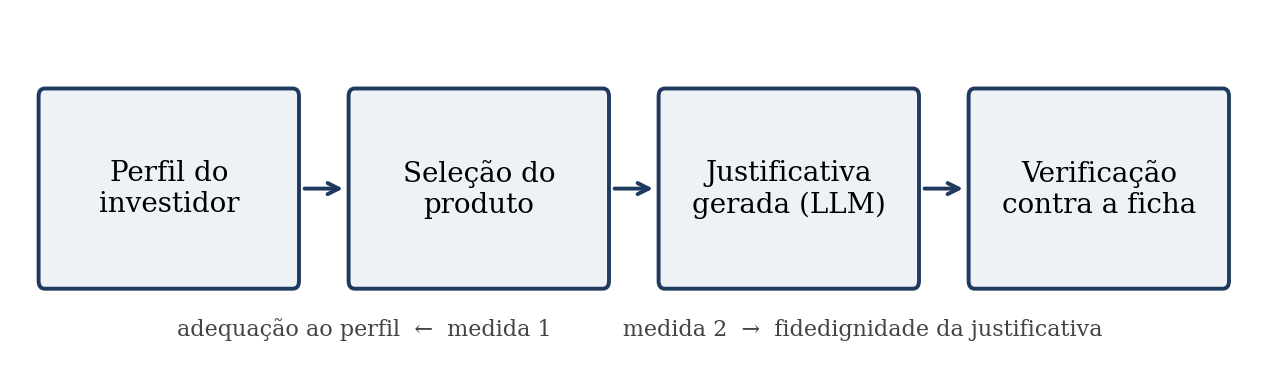
\includegraphics[width=0.9\textwidth]{figuras/fluxo-recomendador.png}
  \fonte{Elaborado pela autora (2026).}
\end{figure}
